% !TeX root = surprises.tex

\chapter{The Axioms of Origami}\label{c.origami-axioms}

%%%%%%%%%%%%%%%%%%%%%%%%%%%%%%%%%%%%%%%%%%%%%%%%%%%%%%%%%%%%%%%

Origami, die Kunst des Papierfaltens, wurde vor mehreren Jahrhunderten in Japan entwickelt und hat heute eine weltweite Anhängerschaft. Im späten zwanzigsten Jahrhundert wurde die mathematische Theorie des Origami entwickelt. Ihre Grundlage ist ein Satz von sieben Axiomen, die 
\emph{Huzita-Hatori-Axiome}, benannt nach Humiaki Huzita, der die ersten sechs Axiome formalisierte, und Koshiro Hatori, der das siebte fand. Jacques Justin veröffentlichte alle sieben Axiome einige Jahre vor Huzita und Hatori, und Margherita P. Beloch formulierte das sechste Axiom im Jahr 1936. Dennoch sind die Axiome als die Huzita-Hatori-Axiome bekannt.

In einer Folge von drei Kapiteln werden wir die Mathematik des Origami erkunden. Dieses Kapitel stellt die Axiome vor, Kap.~\ref{c.origami-cube} verbindet Origami mit den Wurzeln von Polynomen und Kap.~\ref{c.origami-constructions} zeigt, dass Konstruktionen mit Origami Probleme lösen können, die mit Lineal und Zirkel unmöglich sind.
 
Dieses Kapitel enthält einen Abschnitt für jedes der sieben Axiome. Im Anschluss an die Erklärung eines Axioms und ein Diagramm der von ihm spezifizierten \emph{fold} werden die Gleichungen der Falte und der Schnittpunkte mit Hilfe der analytischen Geometrie entwickelt. Eine Falte kann auch als \emph{geometrischer Ort} definiert werden, die Menge aller Punkte, die eine bestimmte Eigenschaft erfüllen. Der Begriff "Falten" stammt von der Origami-Operation, bei der ein Stück Papier gefaltet wird, aber hier wird er verwendet, um die geometrische Linie zu bezeichnen, die durch das Falten des Papiers entstehen würde.

Faltungen führen zu \emph{Reflexionen}. Bei einem Punkt $p$ ergibt seine Spiegelung an einer Falte $l$ einen solchen Punkt $p'$, dass $l$ die Mittelsenkrechte des Liniensegments $\overline{pp'}$ ist (Abb.~\ref{f.origami-def}).

\begin{figure}[ht]
\begin{center}
\begin{tikzpicture}[scale=.8]
\coordinate (P1) at (2,2);
\coordinate (P1P) at (6,4);
\coordinate (mid) at (4,3);
\draw[rotate=30] (mid) rectangle +(8pt,8pt);
\coordinate (m1) at ($(P1)!.5!(mid)$);
\coordinate (m2) at ($(mid)!.5!(P1P)$);
\draw[thick] (m1) -- +(120:4pt);
\draw[thick] (m1) -- +(-60:4pt);
\draw[thick] (m2) -- +(120:4pt);
\draw[thick] (m2) -- +(-60:4pt);
\draw[thick] (P1) -- (P1P);
\draw[very thick,dashed] (4.7,1.6) -- node[very near end,right,yshift=4pt] {$l$} (3.5,4);
\vertex{P1};
\vertex{P1P};
\node[above left] at (P1) {$p$};
\node[above left] at (P1P) {$p'$};
\draw[very thick,dotted,->,bend right=50] (2.1,1.9) to (6.05,3.9);
\end{tikzpicture}
\end{center}
\caption{Die Faltung ist die Mittelsenkrechte der Verbindungslinie zwischen einem Punkt und seiner Spiegelung}\label{f.origami-def}
\end{figure}


\section{Axiom 1}\label{s.ax1}


\begin{axiom}
Bei zwei verschiedenen Punkten $p_1=(x_1,y_1)$, $p_2=(x_2,y_2)$ gibt es eine einzige Falte $l$, die durch beide Punkte verläuft (Abb.~\ref{f.origami-axiom1}).
\end{axiom}

\begin{figure}[ht]
\begin{center}
\begin{tikzpicture}[scale=1]
\draw[step=10mm,white!50!black,thin] (-1,-1) grid (8,6);
\draw[thick] (-1,0) -- (8,0);
\draw[thick] (0,-1) -- (0,6);
\foreach \x in {0,...,8}
  \node at (\x-.2,-.2) {\sm{\x}};
\foreach \y in {1,...,6}
  \node at (-.2,\y-.3) {\sm{\y}};
\coordinate (P1) at (2,2);
\coordinate (P2) at (6,4);
\draw[very thick,dashed] ($(P1)!-.75!(P2)$) -- node[very near end,below] {$l$} ($(P1)!1.5!(P2)$);
\vertex{P1};
\vertex{P2};
\node[above left] at (P1) {$p_1$};
\node[above left] at (P2) {$p_2$};

\draw[very thick,dotted,->,bend left=30] (2,5) to (4,1);
\end{tikzpicture}
\end{center}
\caption{Axiom $1$}\label{f.origami-axiom1}
\end{figure}

\textbf{Ableitung der Gleichung der Falte:}
Die Gleichung der Falte $l$ ergibt sich aus den Koordinaten von $p_1$ und $p_2$. Die Steigung ist der Quotient aus den Differenzen der Koordinaten und der Achsenabschnitt ergibt sich aus $p_1$:
\begin{align}
y - y_1 = \frac{y_2-y_1}{x_2-x_1}(x-x_1)\,.
\end{align}

\begin{example}
Es sei $p_1=(2,2), p_2=(6,4)$. Die Gleichung von $l$ sei:
\begin{eqnarray*}
y-2&=&\frac{4-2}{6-2}(x-2)\\
y&=&\frac{1}{2}x+1\,.
\end{eqnarray*}
\end{example}

%%%%%%%%%%%%%%%%%%%%%%%%%%%%%%%%%%%%%%%%%%%%%%%%%%%%%%%%%%%%%%%%


\section{Axiom 2}\label{s.ax2}



\begin{axiom}
Bei zwei verschiedenen Punkten $p_1=(x_1,y_1)$, $p_2=(x_2,y_2)$ gibt es eine eindeutige Faltung $l$, die $p_1$ auf $p_2$ legt (Abb.~\ref{f.origami-axiom2}).
\end{axiom}

Die Falte ist der geometrische Ort aller Punkte, die äquidistant von $p_1$ und $p_2$.

\begin{figure}[ht]
\begin{center}
\begin{tikzpicture}[scale=1]
\draw[step=10mm,white!50!black,thin] (-1,-1) grid (8,6);
\draw[thick] (-1,0) -- (8,0);
\draw[thick] (0,-1) -- (0,6);
\foreach \x in {0,...,8}
  \node at (\x-.2,-.2) {\sm{\x}};
\foreach \y in {1,...,6}
  \node at (-.2,\y-.3) {\sm{\y}};
\coordinate (P1) at (2,2);
\coordinate (P2) at (6,4);
\coordinate (mid1) at ($(P1)!.5!(P2)$);
\coordinate (mid2) at ($(P1)!.5!(P2)+(-1,2)$);

\draw[rotate=30] (mid1) rectangle +(8pt,8pt);

\draw (P1) -- (P2);
\draw[very thick,dashed] ($(mid1)!-1.4!(mid2)$) -- node[very near end,left,yshift=-12pt] {$l$} ($(mid1)!1.4!(mid2)$);
\vertex{P1};
\vertex{P2};
\node[above left] at (P1) {$p_1$};
\node[above left] at (P2) {$p_2$};

\draw[very thick,dotted,->,bend right=50] (2.1,1.9) to (6,3.9);
\end{tikzpicture}
\end{center}
\caption{Axiom $2$}\label{f.origami-axiom2}
\end{figure}

\noindent\textbf{Herleitung der Gleichung der Faltung:}
Die Faltung $l$ ist die Mittelsenkrechte von $\overline{p_1p_2}$. Ihre Steigung ist der negative Kehrwert der Steigung der Verbindungslinie zwischen $p_1$ und $p_2$. $l$ geht durch den Mittelpunkt zwischen den beiden Punkten:
\begin{align}
y - \frac{y_1+y_2}{2} = -\frac{x_2-x_1}{y_2-y_1}\left(x-\frac{x_1+x_2}{2}\right)\,.\label{eq.midpoint1}
\end{align}

\begin{example}
Es sei $p_1=(2,2), p_2=(6,4)$. Die Gleichung von $l$ sei:
\begin{eqnarray*}
y-\left(\frac{2+4}{2}\right)&=&-\frac{6-2}{4-2}\left(x-\left(\frac{2+6}{2}\right)\right)\\
y&=&-2x+11\,.
\end{eqnarray*}
\end{example}

%%%%%%%%%%%%%%%%%%%%%%%%%%%%%%%%%%%%%%%%%%%%%%%%%%%%%%%%%%%%%%%%

\section{Axiom 3}\label{s.ax3}


\begin{axiom}
Bei zwei Linien $l_1,l_2$ gibt es eine Falte $l$, die $l_1$ auf $l_2$ legt (Abb.~\ref{f.origami-axiom3}).
\end{axiom}
Die Faltung ist der geometrische Ort der Punkte, die von $l_1$ und $l_2$ gleich weit entfernt sind, wobei der Abstand eines Punktes zu einer Geraden die Länge des Geradenstücks ist, das durch den Punkt geht und senkrecht auf der Geraden steht. Mit Hilfe kongruenter Dreiecke lässt sich leicht zeigen, dass die Falte eine Winkelhalbierende des von $l_1$ und $l_2$ gebildeten Winkels ist.

\begin{figure}[ht]
\begin{center}
\begin{tikzpicture}[scale=1]
\draw[step=10mm,white!50!black,thin] (-1,-1) grid (8,7);
\draw[thick] (-1,0) -- (8,0);
\draw[thick] (0,-1) -- (0,7);
\foreach \x in {0,...,8}
  \node at (\x-.2,-.2) {\sm{\x}};
\foreach \y in {1,...,7}
  \node at (-.2,\y-.3) {\sm{\y}};
\coordinate (L1a) at (2,2);
\coordinate (L1b) at (4,6);
\draw (L1a) -- node[very near start,right,yshift=-4pt] {$l_1$} (L1b);
\draw[name path=l1] ($(L1a)!-.75!(L1b)$) -- ($(L1a)!1.25!(L1b)$);
\coordinate (L2a) at (7,1);
\coordinate (L2b) at (4,4);
\draw (L2a) -- (L2b);
\draw[name path=l2] ($(L2a)!-.3!(L2b)$) -- node[very near start,above,xshift=4pt,yshift=2pt] {$l_2$} ($(L2a)!2!(L2b)$);
\path [name intersections = {of = l1 and l2, by = {PM}}];
\node[below left,xshift=-9pt,yshift=-7pt] at (PM) {$p_i$};

\node[above right,xshift=10pt,yshift=4pt] at (PM) {$\alpha$};
\node[below right,xshift=10pt] at (PM) {$\alpha$};
\node[above left,xshift=-3pt,yshift=12pt] at (PM) {$\beta$};
\node[above right,xshift=-3pt,yshift=12pt] at (PM) {$\beta$};

\coordinate (B1a) at (0,4.13);
\coordinate (B1b) at (6,5.1);
\draw[very thick,dashed] ($(B1a)!-.15!(B1b)$) -- node[very near start,above] {$l_{f_1}$}  ($(B1a)!1.35!(B1b)$);

\coordinate (B2a) at (3,6.73);
\coordinate (B2b) at (4,.57);
\draw[very thick,dashed] ($(B2a)!-.05!(B2b)$) -- node[very near end,right,xshift=4pt,yshift=6pt] {$l_{f_2}$} ($(B2a)!1.25!(B2b)$);

\draw[very thick,dotted,->,bend right=50] (6,2.2) to (4.5,6.7);
\draw[very thick,dotted,->,bend left=50] (6.2,1.6) to (1.8,1.3);
\end{tikzpicture}
\end{center}
\caption{Axiom $3$}\label{f.origami-axiom3}
\end{figure}

\noindent\textbf{Herleitung der Gleichung der Faltung:}

\noindent\textit{$l_1,l_2$ sind parallel:} Sei $l_1$ gleich $y=mx+b_1$ und $l_2$ gleich $y=mx+b_2$. Die Falte ist die zu $l_1$ und $l_2$ parallele Linie, die in der Mitte zwischen ihnen liegt:
\[
y=mx+\frac{b_1+b_2}{2}\,.
\]
\noindent\textit{$l_1,l_2$ schneiden sich:} Sei $l_1$ gleich $y=m_1x+b_1$ und $l_2$ gleich $y=m_2x+b_2$. $p_i=(x_i,y_i)$, der Schnittpunkt der beiden Geraden, sei:
\begin{eqnarray*}
m_1x_i+b_1&=&m_2x_i+b_2\\
x_i &=& \frac{b_2-b_1}{m_1-m_2}\\
y_i &=&m_1x_i+b_1\,.
\end{eqnarray*}

\begin{example}\label{ex.axiom3}
Sei $l_1$ gleich $y=2x-2$ und $l_2$ gleich $y=-x+8$. Dann sei $p_i=(x_i,y_i)$:
\begin{eqnarray*}
x_i&=&\frac{8-(-2)}{2-(-1)}=\frac{10}{3}\approx 3.33\\
y_i &=& 2\cdot\frac{10}{3}-2=\frac{14}{3}\approx 4.67\,.
\end{eqnarray*}
\end{example}


Die Faltung ist die Winkelhalbierende des Winkels, den $l_1$ und $l_2$ in ihrem Schnittpunkt bilden. Es gibt zwei mögliche Faltungen, da es zwei Paare von vertikalen Winkeln gibt. Wir müssen die Steigungen der Winkelhalbierenden bestimmen. Ist der Winkel der Geraden $l_1$ zur $x$-Achse $\theta_1$ und der Winkel der Geraden $l_2$ zur $x$-Achse $\theta_2$, so ist die Faltung diejenige, die zur $x$-Achse einen Winkel von $\theta_b=(\theta_1+\theta_2)/2$ bildet.

Es sei $m_1=\tan\theta_1, m_2=\tan \theta_2$. Nach Thm.~\ref{thm.tangent-sum} ist $m_s$, die Steigung der Geraden, die einen Winkel von $\theta_1+\theta_2$ relativ zur $x$-Achse bildet, gleich:
\[
m_s=\tan(\theta_1+\theta_2)= \frac{\tan\theta_1+\tan\theta_2}{1-\tan\theta_1\tan\theta_2}=\frac{m_1+m_2}{1-m_1m_2}\,.
\]
Nach Thm.~\ref{thm.tangent-half} ist $m_b$, die Steigung der Winkelhalbierenden, gleich:
\[
m_b= \tan\frac{\theta_1+\theta_2}{2}=\frac{-1\pm\sqrt{1+\tan^2(\theta_1+\theta_2)}}{\tan (\theta_1+\theta_2)}=\frac{-1\pm\sqrt{1+m_s^2}}{m_s}\,.
\]
\begin{example}
Für $y=2x-2$ und $y=-x+8$ ist die Steigung der Winkelhalbierenden:
\begin{eqnarray*}
m_s&=&\frac{2+(-1)}{1-(2 \cdot -1)}=\frac{1}{3}\\
m_b&=&\frac{-1\pm\sqrt{1+(1/3)^2}}{1/3}=-3\pm \sqrt{10}\approx -6.16,\; 0.162\,.
\end{eqnarray*}
\end{example}

Leiten wir die Gleichung der Falte $l_{f_1}$ mit der positiven Steigung her. Aus Beispiel~\ref{ex.axiom3} sind die Koordinaten des Schnittpunktes der beiden Geraden $(10/3, 14/3)$. Daraus folgt:
\begin{eqnarray*}
\frac{14}{3} &=& (-3+\sqrt{10}) \cdot \frac{10}{3} + b_i\\ b_i&=&\frac{44-10\sqrt{10}}{3}\\
y&=& (-3+\sqrt{10})x + \frac{44-10\sqrt{10}}{3}\approx 0.162x+4.13\,.
\end{eqnarray*}

%%%%%%%%%%%%%%%%%%%%%%%%%%%%%%%%%%%%%%%%%%%%%%%%%%%%%%%%%%%%%%%%

\section{Axiom 4}\label{s.ax4}


\begin{axiom}
Bei einem Punkt $p_1$ und einer Linie $l_1$ gibt es eine einzige Falte $l$ senkrecht zu $l_1$, die durch den Punkt $p_1$ geht (Abb.~\ref{f.origami-axiom4}).
\end{axiom}

Die Falte ist der geometrische Ort aller Punkte auf der Senkrechten zu $l_1$, die durch $p_1$ geht.

\begin{figure}[ht]
\begin{center}
\begin{tikzpicture}[scale=1]
\draw[step=10mm,white!50!black,thin] (-1,-1) grid (8,7);
\draw[thick] (-1,0) -- (8,0);
\draw[thick] (0,-1) -- (0,7);
\foreach \x in {0,...,8}
  \node at (\x-.2,-.2) {\sm{\x}};
\foreach \y in {1,...,7}
  \node at (-.2,\y-.3) {\sm{\y}};
\coordinate (L1a) at (2,0);
\coordinate (L1b) at (5,6);
\draw (L1a) -- node[very near start,right,yshift=-4pt] {$l_1$} ($(L1a)!1.15!(L1b)$);
\coordinate (P1) at (2,6);
\vertex{P1};
\node[above right] at (P1) {$p_1$};
\draw[thick,dashed] (0,7) -- node[very near end,above right] {$l$} (8,3);
\coordinate (intersection) at (4.4,4.8);
\draw[rotate=-30] (intersection) rectangle +(8pt,8pt);

\draw[very thick,dotted,->,bend left=50] (5.4,6.3) to (3.7,3);
\end{tikzpicture}
\end{center}
\caption{Axiom $4$}\label{f.origami-axiom4}
\end{figure}

\noindent\textbf{Herleitung der Gleichung der Falte:}
$l_1$ sei $y = m_1x + b_1$ und $p_1=(x_1,y_1)$. $l$ steht senkrecht auf $l_1$, seine Steigung ist also $-(1/m_1)$. Da sie durch $p_1$ geht, können wir den Achsenabschnitt $b$ berechnen und seine Gleichung aufschreiben:
\begin{eqnarray*}
y_1&=&-\frac{1}{m} x_1 + b\\
b&=& \frac{(my_1+x_1)}{m}\\
y&=&-\frac{1}{m} x +\frac{(my_1+x_1)}{m}\,.
\end{eqnarray*}
\begin{example}
Let $p_1=(2,6)$ and let $l_1$ be $y=2x-4$. The equation of the fold $l$ is:
\[
y=-\frac{1}{2}x + \frac{2\cdot 6 + 2}{2}=-\frac{1}{2}x + 7\,.
\]
\end{example}

%%%%%%%%%%%%%%%%%%%%%%%%%%%%%%%%%%%%%%%%%%%%%%%%%%%%%%%%%%%%%%%%

\section{Axiom 5}\label{s.ax5}


\begin{axiom}
Bei zwei Punkten $p_1,p_2$ und einer Linie $l_1$ gibt es eine Falte $l$, die $p_1$ auf $l_1$ legt und durch $p_2$ geht (Abb.~\ref{f.origami-axiom5}).
\end{axiom}

Da die Falte durch $p_2$ geht und $p_2$ auf der Mittelsenkrechten von $\overline{p_1p_1'}$ liegt, ist die geometrische Ortskurve der Spiegelung von $p_1$ der durch $p_2$ zentrierte Kreis mit dem Radius $\overline{p_1p_2}$. Die Faltung ist so beschaffen, dass die Spiegelung $p_1'$ auf der gegebenen Linie $l_1$ liegt.

\begin{figure}[ht]
\begin{center}
\begin{tikzpicture}[scale=1]
\draw[step=10mm,white!50!black,thin] (-1,-1) grid (9,9);
\draw[thick] (-1,0) -- (9,0);
\draw[thick] (0,-1) -- (0,9);
\foreach \x in {0,...,9}
  \node at (\x-.2,-.2) {\sm{\x}};
\foreach \y in {1,...,9}
  \node at (-.2,\y-.3) {\sm{\y}};
\coordinate (L1a) at (0,3);
\coordinate (L1b) at (8,-1);
\draw (L1a) -- node[near end,below right,xshift=8pt,yshift=-8pt] {$l_1$} (L1b);
\coordinate (P1) at (2,8);
\coordinate (P2) at (4,4);
\vertex{P1};
\vertex{P2};
\node[above left] at (P1) {$p_1$};
\node[above left,yshift=4pt] at (P2) {$p_2$};


\draw[name path=L1] (8,-1) -- (-1,3.5);
\node[draw,name path = circle] at (P2)
    [circle through = (P1)] {};

\path [name intersections = {of = circle and L1, by = {P1P,P1PP}}];
\vertex{P1P};
\vertex{P1PP};
\node[above left,xshift=-2pt,yshift=4pt] at (P1P) {$p_1'$};
\node[above left,yshift=6pt] at (P1PP) {$p_1''$};

\coordinate (f1) at (0,6);
\draw[thick,dashed] ($(f1)!-.25!(P2)$) -- node[very near end,above] {$l_{f_2}$} ($(f1)!2.25!(P2)$);
\coordinate (f2) at (0,2);
\draw[thick,dashed] ($(f2)!-.25!(P2)$) -- node[very near end,below,yshift=-2pt] {$l_{f_1}$} ($(f2)!2.25!(P2)$);

\draw[very thick,dotted,->,bend left=50] (2.1,7.9) to (-.3,3.2);
\draw[very thick,dotted,->,bend left=50] (2.2,7.95) to (6.05,.1);
\end{tikzpicture}
\end{center}
\caption{Axiom $5$}\label{f.origami-axiom5}
\end{figure}

\noindent\textbf{Herleitung der Gleichungen der Faltungen:}
Sei $l_1$ gleich $y=m_1x + b_1$ und sei $p_1=(x_1,y_1)$, $p_2=(x_2,y_2)$. Die Gleichung des in $p_2$ zentrierten Kreises mit dem Radius $\overline{p_1p_2}$ lautet:
\begin{eqnarray*}
(x-x_2)^2 + (y-y_2)^2 = r^2\,,\quad \textrm{where}\\
r^2= (x_2-x_1)^2 + (y_2-y_1)^2\,.
\end{eqnarray*}
Setzt man die Gleichung von $l_1$ in die Gleichung für den Kreis ein, so erhält man:
\begin{eqnarray*}
(x-x_2)^2+((m_1x+b_1)-y_2)^2&=&r^2\\
(x-x_2)^2+(m_1x+(b_1-y_2))^2&=&r^2\,,
\end{eqnarray*}
und wir erhalten eine quadratische Gleichung für die $x$-Koordinaten der möglichen Schnittpunkte:
\begin{align}
x^2(1+m_1^2) \,+\, 2(-x_2+m_1(b-y_2))x \,+\,(x_2^2 + (b_1^2 - 2b_1y_2+y_2^2)-r^2)=0\,.\label{eq.intersections}
\end{align}
Da eine quadratische Gleichung höchstens zwei Lösungen hat, kann es für ein gegebenes Paar von Punkten und eine Linie null, eine oder zwei Falten geben. Aus den Lösungen $x_1',x_1''$ können wir $y_1',y_1''$ aus $y=m_1x+b_1$ berechnen. Die reflektierten Punkte sind $p_1'=(x_1',y_1')$, $p_1''=(x_1'',y_1'')$.
\begin{example}
Es sei $p_1=(2,8)$, $p_2=(4,4)$ und $l_1$ sei $y=-\frac{1}{2}x +3$. Die Gleichung des Kreises ist $(x-4)^2 + (y-4)^2 = (4-2)^2+(4-8)^2=20$. Setzt man die Geradengleichung in die Kreisgleichung ein, so erhält man eine quadratische Gleichung für die $x$-Koordinaten der Schnittpunkte (oder man verwendet Gl.~\ref{eq.intersections}):
\begin{eqnarray*}
(x-4)^2 + \left(\left(-\frac{1}{2}x+3\right)-4\right)^2&=&20\\
(x-4)^2 + (-1)^2\cdot\left(\frac{1}{2}x+1\right)^2-20&=&0\\
5x^2 -28x -12&=&0\\
(5x+2)(x-6)&=&0\,.
\end{eqnarray*}
Die beiden Kreuzungspunkte sind:
\[
p_1'=(-2/5,16/5) = (-0.4,3.2)\,,\quad p_1''=(6,0)\,.
\]
\end{example}
Die Falten sind die Winkelhalbierenden von $\overline{p_1p_1'}$ und $\overline{p_1p_1''}$.
\begin{example}
Für $p_1=(2,8)$ und $p_1'=(-2/5,16/5)$ lautet die Gleichung von $l_{f_1}$:
\begin{eqnarray*}
y-\frac{8+(16/5)}{2}&=&-\frac{(-2/5)-2}{(16/5)-8}\left(x-\frac{2+\left(-2/5\right)}{2}\right)\\
y&=&-\frac{1}{2}x+6\,.
\end{eqnarray*}
\end{example}

\begin{example}
Für $p_1=(2,8)$ und $p_1''=(6,0)$ lautet die Gleichung von $l_{f_2}$:
\begin{eqnarray*}
y-\frac{8+0}{2}&=&-\frac{6-2}{0-8}\left(x-\frac{2+6}{2}\right)\\
y&=&\frac{1}{2}x+2\,.
\end{eqnarray*}
\end{example}

%%%%%%%%%%%%%%%%%%%%%%%%%%%%%%%%%%%%%%%%%%%%%%%%%%%%%%%%%%%%%%%%

\section{Axiom 6}\label{s.ax6}

\begin{axiom}
Bei zwei Punkten $p_1,p_2$ und zwei Geraden $l_1,l_2$ gibt es eine Falte $l$, die $p_1$ auf $l_1$ und $p_2$ auf $l_2$ legt (Abb.~\ref{f.origami-axiom6}).
\end{axiom}

Eine Faltung, die $p_i$ auf $l_i$ legt, ist eine solche Linie $l_f$, dass der Abstand von $p_i$ zu $l_f$ gleich dem Abstand ihrer Spiegelung $p_i'$ von $l_f$ ist. Die geometrische Ortskurve der Punkte, die von einem Punkt $p_i$ und einer Geraden $l_i$ gleich weit entfernt sind, ist eine \emph{parabola}. $p_i$ heißt der \emph{focus} und $l_1$ heißt der \emph{directrix}. Eine Falte ist eine beliebige Linie, die die Parabel tangiert (Sect.~\ref{s.parabola}).

\begin{figure}[ht]
\begin{center}
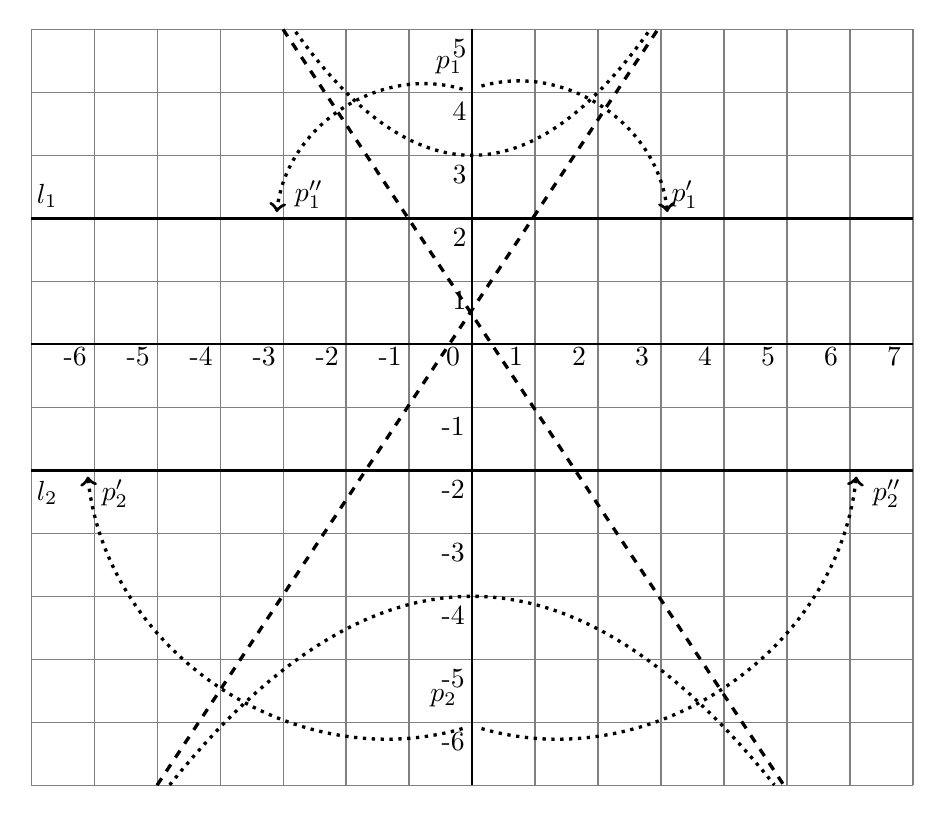
\begin{tikzpicture}[scale=.8]
\draw[step=10mm,white!50!black,thin] (-7,-7) grid (7,5);
\draw[thick] (-7,0) -- (7,0);
\draw[thick] (0,-7) -- (0,5);
\foreach \x in {-6,...,7}
  \node at (\x-.3,-.2) {\sm{\x}};
\foreach \y in {1,...,5}
  \node at (-.2,\y-.3) {\sm{\y}};
\foreach \y in {-6,...,-1}
  \node at (-.3,\y-.3) {\sm{\y}};
  
\coordinate (P1) at (0,4);
\coordinate (P2) at (0,-6);
\coordinate (P1P) at (3.1,2);
\coordinate (P2P) at (-6.12,-2);
\coordinate (P1PP) at (-3.1,2);
\coordinate (P2PP) at (6.12,-2);

\vertex{P1};
\vertex{P2};
\vertex{P1P};
\vertex{P2P};
\vertex{P1PP};
\vertex{P2PP};

\node[above left,yshift=3pt] at (P1) {$p_1$};
\node[above left,xshift=-2pt,yshift=2pt] at (P2) {$p_2$};
\node[above right,xshift=-2pt] at (P1P) {$p_1'$};
\node[below right,xshift=2pt] at (P2P) {$p_2'$};
\node[above right,xshift=3pt] at (P1PP) {$p_1''$};
\node[below right,xshift=2pt] at (P2PP) {$p_2''$};

\draw[very thick] (-7,2) -- node[very near start,above,xshift=-34pt] {$l_1$} (7,2);
\draw[very thick] (-7,-2) -- node[very near start,below,xshift=-34pt] {$l_2$} (7,-2);

\draw[domain=-4.8:4.8,samples=50,very thick,dotted] plot (\x,{-.13*\x*\x-4});
\draw[domain=-2.8:2.8,samples=50,very thick,dotted] plot (\x,{.25*\x*\x+3});

\draw[very thick,dashed] (-5,-7) -- (2.95,5);
\draw[very thick,dashed] (-3,5) -- (4.95,-7);

\draw[very thick,dotted,->,bend left=50] (.15,4.1) to (3.1,2.1);
\draw[very thick,dotted,->,bend right=50] (-.15,4.05) to (-3.1,2.1);

\draw[very thick,dotted,->,bend right=50] (.15,-6.1) to (6.1,-2.1);
\draw[very thick,dotted,->,bend left=50] (-.15,-6.1) to (-6.1,-2.1);

\end{tikzpicture}
\end{center}
\caption{Axiom $6$}\label{f.origami-axiom6}
\end{figure}

Damit eine Falte gleichzeitig $p_1$ auf $l_1$ und $p_2$ auf $l_2$ legen kann, muss sie eine gemeinsame Tangente an die beiden Parabeln sein. Es kann null, eine, zwei oder drei gemeinsame Tangenten geben (Abb.~\ref{f.two-para-1-zero}, \ref{f.two-para-1-one}, \ref{f.two-para-1-two}, \ref{f.two-para-1-three}).
\begin{figure}[ht]
\begin{minipage}{.45\textwidth}
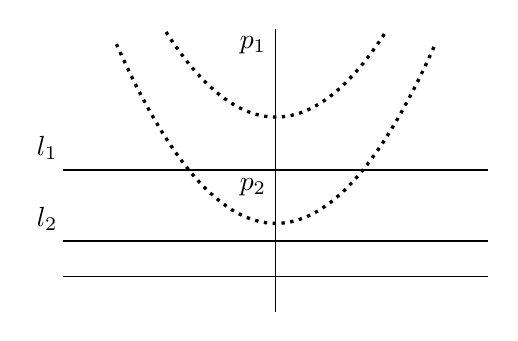
\begin{tikzpicture}[scale=.45]
\draw (-6,0) -- (6,0);
\draw (0,-1) -- (0,7);
\coordinate (P1) at (0,6);
\coordinate (P2) at (0,2);
\vertex{P1};
\vertex{P2};
\node[above left] at (P1) {$p_1$};
\node[above left] at (P2) {$p_2$};
\draw[thick] (-6,3) -- node[very near start,above,xshift=-25pt] {$l_1$} (6,3);
\draw[thick] (-6,1) -- node[very near start,above,xshift=-25pt] {$l_2$} (6,1);
\draw[domain=-3.1:3.1,samples=50,very thick,dotted] plot (\x,{.25*\x*\x+4.5});
\draw[domain=-4.5:4.5,samples=50,very thick,dotted] plot (\x,{.25*\x*\x+1.5});
\end{tikzpicture}
\caption{Keine gemeinsamen Berührungspunkte}\label{f.two-para-1-zero}
\end{minipage}
\hfill
\begin{minipage}{.45\textwidth}
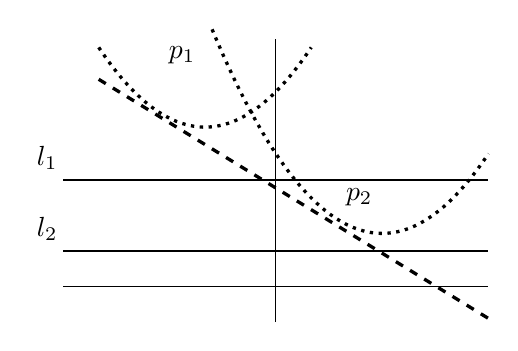
\begin{tikzpicture}[scale=.45]
\draw (-6,0) -- (6,0);
\draw (0,-1) -- (0,7);
\coordinate (P1) at (-2,6);
\coordinate (P2) at (3,2);
\vertex{P1};
\vertex{P2};
\node[above left] at (P1) {$p_1$};
\node[above left] at (P2) {$p_2$};
\draw[thick] (-6,3) -- node[very near start,above,xshift=-25pt] {$l_1$} (6,3);
\draw[thick] (-6,1) -- node[very near start,above,xshift=-25pt] {$l_2$} (6,1);
\draw[domain=-5:1,samples=50,very thick,dotted] plot (\x,{.25*(\x+2)*(\x+2)+4.5});
\draw[domain=-1.8:6,samples=50,very thick,dotted] plot (\x,{.25*(\x-3)*(\x-3)+1.5});
\draw[very thick,dashed] (-5,5.85) -- (6,-.9);
\end{tikzpicture}
\caption{Eine gemeinsame Tangente}\label{f.two-para-1-one}
\end{minipage}
\end{figure}

\begin{figure}[ht]
\begin{minipage}{.45\textwidth}
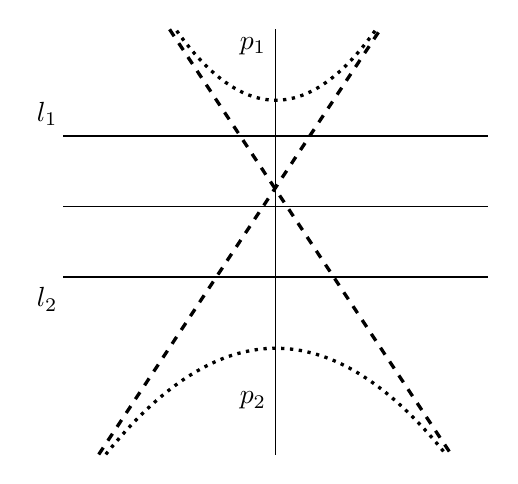
\begin{tikzpicture}[scale=.45]
\draw (-6,0) -- (6,0);
\draw (0,-7) -- (0,5);
\coordinate (P1) at (0,4);
\coordinate (P2) at (0,-6);
\vertex{P1};
\vertex{P2};
\node[above left] at (P1) {$p_1$};
\node[above left] at (P2) {$p_2$};
\draw[thick] (-6,2) -- node[very near start,above,xshift=-25pt] {$l_1$} (6,2);
\draw[thick] (-6,-2) -- node[very near start,below,xshift=-25pt] {$l_2$} (6,-2);
\draw[domain=-4.8:4.8,samples=50,very thick,dotted] plot (\x,{-.13*\x*\x-4});
\draw[domain=-2.8:2.8,samples=50,very thick,dotted] plot (\x,{.25*\x*\x+3});
\draw[very thick,dashed] (-5,-7) -- (2.95,5);
\draw[very thick,dashed] (-3,5) -- (4.95,-7);
\end{tikzpicture}
\caption{Zwei gemeinsame Berührungspunkte}\label{f.two-para-1-two}
\end{minipage}
\hfill
\begin{minipage}{.45\textwidth}
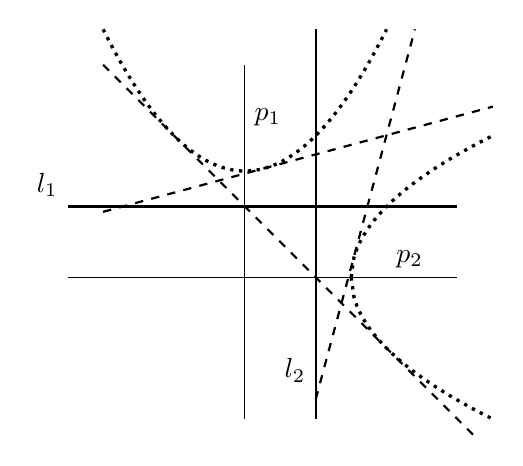
\begin{tikzpicture}[scale=.45]
\draw (-5,0) -- (6,0);
\draw (0,-4) -- (0,6);
\coordinate (P1) at (0,4);
\coordinate (P2) at (4,0);
\vertex{P1};
\vertex{P2};
\node[above right] at (P1) {$p_1$};
\node[above right] at (P2) {$p_2$};
\draw[thick] (-5,2) -- node[very near start,above,xshift=-25pt] {$l_1$} (6,2);
\draw[thick] (2,-4) -- node[very near start,left] {$l_2$} (2,7);
\draw[domain=-4:4,samples=50,very thick,dotted] plot (\x,{.25*\x*\x+3});
\draw[domain=3:7,samples=50,very thick,dotted] plot (\x,{sqrt(4*\x-12)});
\draw[domain=3:7,samples=50,very thick,dotted] plot (\x,{-sqrt(4*\x-12)});

\draw[thick,dashed,domain=-4:6.5] plot (\x,-\x+2);
\draw[thick,dashed,domain=-4:7] plot (\x,.27*\x+2.93);
\draw[thick,dashed,domain=2:4.8] plot (\x,3.73*\x-10.9);
\end{tikzpicture}
\end{minipage}
\caption{Drei gemeinsame Berührungspunkte}\label{f.two-para-1-three}
\end{figure}

Die Formel für eine beliebige Parabel ist recht komplex, so dass wir uns bei der Darstellung auf Parabeln beschränken, deren Symmetrieachse die $x$- oder $y$-Achse ist.

\subsection{Herleitung der Gleichung einer Falte}

Sei $(0,f)$ der Brennpunkt einer Parabel mit der Leitkurve $y=d$. Definieren Sie $p=f-d$, die vorzeichenbehaftete Länge des Streckenabschnitts zwischen dem Brennpunkt und der Leitkurve.\footnote{Wir haben die Notation $p_i$ für Punkte verwendet; die Verwendung von $p$ hier könnte verwirrend sein, aber es ist die Standardnotation. Der formale Name für $p$ ist die Hälfte des \emph{latus rectum}.} Wenn der Scheitelpunkt der Parabel auf der $x$-Achse liegt, lautet die Gleichung der Parabel $y=x^2/2p$. Um die Parabel auf der $y$-Achse nach oben oder unten zu verschieben, so dass ihr Scheitelpunkt bei $(0,h)$ liegt, addiert man $h$ zur Gleichung der Parabel (Abb.~\ref{f.elements-parabola}):
\[y=\frac{x^2}{2p}+h\,.\]

\begin{figure}[htb]
\begin{center}
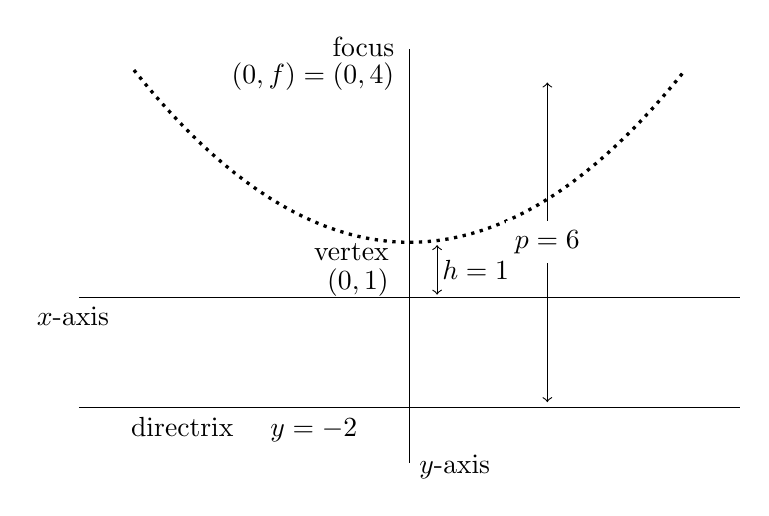
\begin{tikzpicture}[scale=.7]
\draw (-6,0) -- node[very near start,below,xshift=-32pt] {$x$-\textrm{axis}}(6,0);
\draw (0,-3) -- node[very near start,right,yshift=-20pt] {$y$-\textrm{axis}}(0,4.5);
\draw (-6,-2) -- node[near start,below] {\textrm{directrix} $\quad y=-2$} (6,-2);
\draw[domain=-5:5,samples=50,very thick,dotted] plot (\x,{\x*\x/8+1});
\coordinate (F) at (0,4);
\coordinate (V) at (0,1);
\coordinate (Y) at (0,-2);
\vertex{F};
\node[left,xshift=-2pt,yshift=0pt] at (F) {$(0,f)=(0,4)$}; \node[above left,xshift=-2pt,yshift=4pt] at (F) {\textrm{focus}};
\node[below left,xshift=-4,yshift=3pt] at (V) {\textrm{vertex}};
\node[below left,xshift=-4,yshift=-6pt] at (V) {$(0,1)$};
\draw[<->] (2.5,-1.9) -- node[fill=white] {$p=6$} +(0,5.8);
\draw[<->] (.5,.05) -- +(0,.9);
\node at (1.2,.5) {$h=1$} +(0,.9);
\end{tikzpicture}
\end{center}
\caption{Die Elemente der Definition einer Parabel}\label{f.elements-parabola}
\end{figure}
Definieren Sie $a=2ph$ so, dass die Gleichung der Parabel lautet:
\begin{subeqnarray}
y&=&\frac{x^2}{2p}+\frac{a}{2p}\\
x^2-2py+a&=&0\,.\slabel{eq.eq-parabola}
\end{subeqnarray}
Die Gleichung der Parabel in Abb.~\ref{f.elements-parabola} ist $x^2-12y +12=0$.

Setzt man die Gleichung einer beliebigen Geraden $y=mx+b$ in Gl.~\ref{eq.eq-parabola} ein, erhält man eine Gleichung für die Schnittpunkte der Geraden und der Parabel:
\begin{eqnarray*}
x^2-2p(mx+b)+a&=&0\\
x^2+(-2mp)x+(-2pb+a)&=&0\,.
\end{eqnarray*}
Die Gerade tangiert die Parabel nur dann, wenn diese quadratische Gleichung genau eine Lösung hat, und nur dann, wenn ihre Diskriminante Null ist:
\begin{subeqnarray}
(-2mp)^2\:-\:4\cdot 1\cdot (-2pb+a)=0\\
m^2p^2+2pb-a=0\,.\slabel{eq.disc}
\end{subeqnarray}
Dies ist eine Gleichung mit den Variablen $m,b$ für die Tangenten an der Parabel. Um die gemeinsamen Tangenten an die beiden Parabeln zu erhalten, müssen wir die Gleichungen für die beiden Parabeln gleichzeitig lösen.

\begin{example}\mbox{}

\noindent\textbf{Parabel 1:} Brennpunkt $(0,4)$, Leitlinie $y=2$, Scheitelpunkt $(0,3)$.

\noindent{}$p=2$, $a=2\cdot 2\cdot 3=12$. Die Gleichung der Parabel lautet:
\[
x^2-4y +12=0\,.
\]
Setzt man $p$ und $a$ in Gl.~\ref{eq.disc} ein und vereinfacht, so erhält man:
\[
m^2+b-3=0\,.
\]

\noindent\textbf{Parabel 2:} Brennpunkt $(0,-4)$, Leitlinie $y=-2$, Scheitelpunkt $(0,-3)$.

\noindent{}$p=-2$, $a=2\cdot -2\cdot -3=12$. Die Gleichung der Parabel lautet:
\[
x^2+4y+12=0\,.
\]
Setzt man $p$ und $a$ in Gl.~\ref{eq.disc} ein und vereinfacht, so erhält man:
\[
m^2-b-3=0\,.
\]
Die Lösungen der beiden Gleichungen:
\begin{eqnarray*}
m^2+b-3&=&0\\
m^2-b-3&=&0
\end{eqnarray*}
are $m=\pm\sqrt{3}\approx \pm 1.73$ and $b=0$. Es gibt zwei gemeinsame Berührungspunkte:
\[
y=\sqrt{3}x\,,\quad y=-\sqrt{3}x\,.
\]
\end{example}

\begin{example}\mbox{}

\noindent\textbf{Parabel 1:}
Unverändert.

\noindent\textbf{Parabel 2:} Brennpunkt $(0,-6)$, Leitlinie $y=-2$, Scheitelpunkt $(0,-4)$.

\noindent{}$p=-4$, $a=2\cdot -4\cdot -4=32$. Die Gleichung der Parabel lautet:
\[
x^2+8y +32=0\,.
\]
Setzt man $p$ und $a$ in Gl.~\ref{eq.disc} ein und vereinfacht, so erhält man:
\[
2m^2-b-4=0\,.
\]
Die Lösungen der beiden Gleichungen:
\begin{eqnarray*}
m^2+b-3&=&0\\
2m^2-b-4&=&0
\end{eqnarray*}
sind $m=\pm\sqrt{\displaystyle\frac{7}{3}}\approx \pm 1.53$ und $b=\displaystyle\frac{2}{3}$. Es gibt zwei gemeinsame Berührungspunkte:
\[
y=\sqrt{\frac{7}{3}}x+\frac{2}{3}\,,\quad y=-\sqrt{\frac{7}{3}}x+\frac{2}{3}\,.
\]
\end{example}

%%%%%%%%%%%%%%%%%%%%%%%%%%%%%%%%%%%%%%%%%%%%%%%%%%%%%%%%%%%%%%%%

\begin{example}\mbox{}

\noindent{}Definieren wir nun eine Parabel, deren Symmetrieachse die $x$-Achse ist.

\noindent\textbf{Parabel 1:} Unverändert. 

\noindent\textbf{Parabel 2:} Brennpunkt $(4,0)$, Leitlinie $x=2$, Scheitelpunkt $(3,0)$.

\noindent{}$p=2$, $a=2\cdot 2\cdot 3=12$. Die Gleichung der Parabel lautet:
\begin{align}
y^2-4x+12 = 0\,.\label{eq.x-symmetry-parabola}
\end{align}
Dies ist eine Gleichung mit $x$ und $y^2$ anstelle von $x^2$ und $y$, so dass Gl.~\ref{eq.disc} nicht verwendet werden kann und wir die Ableitung erneut durchführen müssen.

Setzen Sie die Geradengleichung in Gl.~\ref{eq.x-symmetry-parabola} ein:
\begin{eqnarray*}
(mx+b)^2-4x+12&=&0\\
m^2x^2+(2mb-4)x+(b^2+12)&=&0\,.
\end{eqnarray*}
Setzen Sie die Diskriminante gleich Null und vereinfachen Sie:
\begin{eqnarray*}
(2mb-4)^2\:-\:4m^2(b^2+12)&=&0\\
-3m^2-mb+1&=&0\,.
\end{eqnarray*}
Wenn wir versuchen, die beiden Gleichungen zu lösen:
\begin{eqnarray*}
m^2+b-3&=&0\\
-3m^2-mb+1&=&0\,,
\end{eqnarray*}
erhalten wir eine \emph{kubische} Gleichung mit der Variablen $m$:
\begin{align}
m^3-3m^2-3m+1=0\,.\label{eq.cubic}
\end{align}
Da eine kubische Gleichung mindestens eine und höchstens drei reelle Lösungen hat, kann es eine, zwei oder drei gemeinsame Berührungspunkte geben.

Die Formel für die Lösung allgemeiner kubischer Gleichungen ist ziemlich kompliziert, also habe ich einen Rechner im Internet benutzt und die drei Lösungen ermittelt:
\[m=3.73,\:m=-1,\:m=0.27\,.\]
Aus der Form von Gl.~\ref{eq.cubic} kann man schließen, dass $m=1$ oder $m=-1$ eine Lösung ist:
\begin{eqnarray*}
1^3-3\cdot 1^2-3\cdot 1+1&=&-4\\
(-1)^3-3\cdot (-1)^2-3\cdot(-1)+1&=&0\,.
\end{eqnarray*}
Dividiert man Gl.~\ref{eq.cubic} durch $m-(-1)=m+1$, so erhält man die quadratische Gleichung $m^2-4m+1$, deren Wurzeln die beiden anderen Lösungen der kubischen Gleichung sind $m=2\pm\sqrt{3}\approx 3.73, 0.27$.
\end{example}

%%%%%%%%%%%%%%%%%%%%%%%%%%%%%%%%%%%%%%%%%%%%%%%%%%%%%%%%%%%%%%%%

\subsection{Ableitung der Gleichungen der Reflexionen}

Wir leiten die Lage der Spiegelung $p_1'=(x_1',y_1')$ von $p_1=(x_1,y_1)$ an einer Tangente $l_t$ ab, deren Gleichung $y=m_tx+b_t$ ist. Finden Sie zunächst die Gerade $l_p$ mit der Gleichung $y=m_px+b_p$, die senkrecht auf $l_t$ steht und durch $p_1$ geht:
\begin{eqnarray*}
y&=&-\frac{1}{m_t}x+b_p\\
y_1&=&-\frac{1}{m_t}x_1+b_p\\
y&=&\frac{-x}{m_t}+\left(y_1+\frac{x_1}{m_t}\right)\,.
\end{eqnarray*}
Finden Sie nun den Schnittpunkt $p_t=(x_t,y_t)$ von $l_t$ und $l_p$:
\begin{eqnarray*}
m_tx_t+b_t&=&\frac{-x_t}{m_t}+\left(y_1+\frac{x_1}{m_t}\right)\\
x_t&=&\frac{\left(y_1+\displaystyle\frac{x_1}{m_t}-b_t\right)}{\left(m_t+\displaystyle\frac{1}{m_t}\right)}\\
y_t&=&m_tx_t+b_t\,.
\end{eqnarray*}
$p_t$ ist der Mittelpunkt zwischen $p_1$ und $p_1'$:
\[
\begin{array}{rcl@{\hspace{3ex}}rcl}
x_t&=&\displaystyle\frac{x_1+x_1'}{2}\,, &x_1'&=&2x_t-x_1\,,\\
y_t&=&\displaystyle\frac{y_1+y_1'}{2}\,,& y_1'&=&2y_t-y_1\,.
\end{array}
\]
\begin{example}
Sei $l_t$ $y=\sqrt{3}x+0$ und sei $p_1=(0,4)$:
\begin{eqnarray*}
x_t&=&\frac{\left(4+\displaystyle\frac{0}{\sqrt{3}}-0\right)}{\left(\sqrt{3}+\displaystyle\frac{1}{\sqrt{3}}\right)}=\sqrt{3}\\
y_t&=&\sqrt{3}\sqrt{3}+0=3\\
x_1'&=&2x_t-x_1=2\sqrt{3}\approx 3.46\\
y_1'&=&2y_t-y_1= 2\,.
\end{eqnarray*}
\end{example}

%%%%%%%%%%%%%%%%%%%%%%%%%%%%%%%%%%%%%%%%%%%%%%%%%%%%%%%%%%%%%%%%

\subsection{Tangenten an eine Parabel}\label{s.parabola}

Wir wollen beweisen, dass die Falten von Axiom~$6$ Tangenten an die Parabeln sind.
Abbildung~\ref{f.parabola-locus} zeigt fünf Punkte
$p_i$, $i=1,\ldots,5$, wobei jeder Punkt $p_i$ sowohl vom Brennpunkt als auch von der Leitlinie einen Abstand $a_i$ hat. Fallen Sie senkrechte Linien von $p_i$ zur Leitkurve und bezeichnen Sie die Schnittpunkte dieser Linien mit der Leitkurve mit $p_i'$. Nach Axiom~$2$ gibt es Falten $l_i$ durch $p_i$, die $p$ auf die Leitkurve legen. Die Punkte $p_i'$ sind die Spiegelungen von $p$ an den Falten. Die Abbildung zeigt die Faltung $l_1$ durch $p_1$ und die Spiegelung $p_1'$.

\begin{figure}[ht]
\begin{center}
\begin{tikzpicture}[scale=.8]
\draw (-6,0) -- node[very near start,below,xshift=-32pt] {$x$-axis} (6,0);
\draw (0,-3) -- node[very near start,right,yshift=-15pt] {$y$-axis} (0,4.5);
\draw[thick] (-6,-2) -- node[near end,below] {directrix $\quad y=-f$} (6,-2);
\draw[domain=-6:6,samples=50,very thick,dotted] plot (\x,{\x*\x/8});
\coordinate (F) at (0,2);
\vertex{F};
\node[above left,xshift=-2pt,yshift=15pt] at (F) {$(0,f)$};
\node[above left,xshift=-5pt,yshift=26pt] at (F) {focus}; \node[above right] at (F) {$p$};
\coordinate (vertex) at (0,0);
\vertex{vertex};
\node[below right] at (vertex) {$p_2$};
\coordinate (FP) at (-5,-2);
\node[below] at (FP) {$p_1'$};
\coordinate (F1) at (2,.5);
\vertex{F1};
\node[below right] at (F1) {$p_3$};
\coordinate (F2) at (3,1.125);
\vertex{F2};
\node[below right] at (F2) {$p_4$};
\coordinate (F3) at (5,3.125);
\vertex{F3};
\node[below right] at (F3) {$p_5$};
\coordinate (F4) at (-5,3.125);
\vertex{F4};
\node[above right] at (F4) {$p_1$};
\draw (F) -- node[left] {$a_2$} (0,0) -- node[left] {$a_2$} (0,-2);
\draw (F) -- node[near end,left] {$a_3$} (F1) -- node[left] {$a_3$} (2,-2);
\draw (F) -- node[near end,above] {$a_4$} (F2) -- node[left] {$a_4$} (3,-2);
\draw (F) -- node[above] {$a_5$} (F3) -- node[left] {$a_5$} (5,-2);
\draw (F) -- node[above] {$a_1$} (F4) -- node[left] {$a_1$} (FP);
\draw[very thick,dashed] ($(F4)!-.4!(-2.5,0)$) -- node[near end,right,xshift=2pt] {$l_1$} ($(F4)!1.8!(-2.5,0)$);
\draw (0,-2) rectangle +(9pt,9pt);
\draw (2,-2) rectangle +(9pt,9pt);
\draw (3,-2) rectangle +(9pt,9pt);
\draw (5,-2) rectangle +(9pt,9pt);
\draw (-5,-2) rectangle +(9pt,9pt);
\end{tikzpicture}
\end{center}
\caption{Die Tangente als geometrische Ortskurve}\label{f.parabola-locus}
\end{figure}

\begin{figure}[thb]
\begin{center}
\begin{tikzpicture}[scale=.8]
\draw[thick] (-6,-2) -- node[near end, below] {$d$} (6,-2);
\draw[domain=-5.5:5.5,samples=50,very thick,dotted] plot (\x,{\x*\x/8});
\coordinate (F) at (0,2);
\vertex{F};
\node[above right] at (F) {$p$};
\coordinate (FP) at (-3,-2);
\node[below] at (FP) {$p'$};
\coordinate (F4) at (-3,1.125);
\vertex{F4};
\node[above right] at (F4) {$r$};
\coordinate (F5) at (-5,2.775);
\vertex{F5};
\node[left,yshift=-4pt] at (F5) {$q$};
\coordinate (F5p) at (-5,-2);
\node[below] at (F5p) {$p''$};
\draw (F) -- node[above] {$b$} (F4) -- node[left] {$b$} (FP);
\draw (F) -- node[above] {$c$} (F5);
\draw (F5) -- node[left] {$e$} (F5p);
\draw[thick,dashed,name path=fold] ($(F4)+(140:4)$) -- (F4) -- node[below,xshift=3pt,yshift=-4pt] {$l$} ($(F4)+(-40:5.3)$);
\draw (FP) rectangle +(10pt,10pt);
\draw (F5p) rectangle +(10pt,10pt);
\draw (F5) -- (FP);
\draw[name path=base] (F) -- (FP);
\path [name intersections = {of = base and fold, by = {G}}];
\node[below,yshift=-4pt] at (G) {$s$};
\draw[rotate=140] (G) rectangle +(10pt,10pt);
\path (FP) -- node[left] {$c$} (F5);
\path (F) -- node[below] {$a$} (G) -- node[below] {$a$} (FP);
\end{tikzpicture}
\end{center}
\caption{Der Beweis, dass die Falte eine Tangente ist}\label{f.tangent-proof}
\end{figure}

\begin{theorem}\label{thm.parabola-tangents}
Die Falten des Axioms~$6$ sind die Tangenten an die Parabeln, die die Orte der Punkte sind, die den Punkten $p_1,p_2$ bzw. $l_l,l_2$ äquidistant sind.
\end{theorem}
\begin{proof}
In Abb.~\ref{f.tangent-proof} ist der Brennpunkt $p$ und die Leitlinie $d$. $p'$ ist ein Punkt auf der Leitlinie und $l$ ist die Falte, die $p$ auf $p'$ spiegelt. Sei $s$ der Schnittpunkt von $\overline{pp'}$ und $l$. Dann sei $\overline{ps}=\overline{p's}=a$ und $l\perp \overline{pp'}$, da $l$ die Mittelsenkrechte von $\overline{pp'}$ ist.

Sei $r$ der Schnittpunkt der Senkrechten $d$ durch $p'$ und die Falte $l$. Dann ist $\triangle psr\cong \triangle p'sr$ durch Seite-Winkel-Seite. Daraus folgt, dass 
$\overline{pr}=\overline{p'r}=b$ also ist $r$ ein Punkt auf der Parabel. Wählen Sie einen Punkt $p''$ auf der Leitkurve, der sich von $p'$ unterscheidet, und nehmen Sie an, dass die Falte $l$ auch $p$ auf $p''$ spiegelt. $q$ sei der Schnittpunkt der Senkrechten zu $d$ durch $p''$ und die Falte $l$. $\triangle psq\cong \triangle p'sq$ so $\overline{pq}=\overline{p'q}=c$. Bezeichne $\overline{qp''}=e$. Wenn $q$ ein Punkt auf der Parabel ist, dann ist $e=\overline{qp''}=\overline{qp}=c$, aber $c$ ist die Hypotenuse des rechtwinkligen Dreiecks $\triangle qp''p'$ und es ist nicht möglich, dass die Hypotenuse gleich einer der anderen Seiten des rechtwinkligen Dreiecks ist. Daher hat die Falte $l$ nur einen Schnittpunkt mit der Parabel und muss eine Tangente sein.
\end{proof}

%%%%%%%%%%%%%%%%%%%%%%%%%%%%%%%%%%%%%%%%%%%%%%%%%%%%%%%%%%%%%%%%

\section{Axiom 7}\label{s.ax7}


\begin{axiom}
Bei einem Punkt $p_1$ und zwei Geraden $l_1$ und $l_2$ gibt es eine Falte $l$, die $p_1$ auf $l_1$ legt und senkrecht auf $l_2$ steht (Abb.~\ref{f.origami-axiom7}).
\end{axiom}

Die Falte ist der geometrische Ort aller Punkte auf der zu $l_2$ senkrechten und von $p_1$ und $p_1'$, der Spiegelung von $p_1$ an $l_1$, äquidistanten Linie.

\smallskip

\noindent\textbf{Herleitung der Gleichung der Faltung:}
Es sei $p_1=(x_1,y_1)$, $l_1$ sei $y = m_1x + b_1$ und $l_2$ sei $y=m_2x+b_2$. Sei $l_p$ die Linie, die $\overline{p_1p_1'}$ enthält. Da $l\perp l_2, l_p\perp l$, folgt, dass $l_p\parallel l_2$ und die Gleichung von $l_p$ $y=m_2x+b_p$ ist.

\begin{figure}[tbh]
\begin{center}
\begin{tikzpicture}[scale=.8]
\draw[step=10mm,white!50!black,thin] (-1,-1) grid (9,8);
\draw[thick] (-1,0) -- (9,0);
\draw[thick] (0,-1) -- (0,8);
\foreach \x in {0,...,9}
  \node at (\x-.2,-.2) {\sm{\x}};
\foreach \y in {1,...,8}
  \node at (-.2,\y-.3) {\sm{\y}};
  
\coordinate (P1) at (5,3);
\node[below left] at (P1) {$p_1$};
\vertex{P1};

\coordinate (P1P) at (2.75,5.25);
\node[left,xshift=-4pt] at (P1P) {$p_1'$};
\vertex{P1P};

\draw (1,0) -- node[very near start,right,xshift=2pt] {$l_1$} (3,6);
\draw[name path=l2] (8,3) -- node[very near start,right,xshift=-2pt,yshift=6pt] {$l_2$} (5,6);

\draw ($(1,0)!-.16!(3,6)$) -- ($(1,0)!1.33!(3,6)$);

\draw ($(8,3)!-.33!(5,6)$) -- ($(8,3)!1.66!(5,6)$);

\draw ($(P1)!-.4!(P1P)$) -- node[very near start,below,yshift=-4pt] {$l_p$} ($(P1)!1.5!(P1P)$);

\draw[very thick,dashed,name path=fold] (-1,-.75) -- node[very near end,above,xshift=4pt,yshift=6pt] {$l$} (7.75,8);

\coordinate (mid) at ($(P1)!.5!(P1P)$);
\node[below,yshift=-8pt] at (mid) {$p_m$};

\path [name intersections = {of = fold and l2, by = {perp}}];
\draw[rotate=-45] (mid) rectangle +(8pt,8pt);
\draw[rotate=-45] (perp) rectangle +(8pt,8pt);


\draw[very thick,dotted,->,bend right=50] (5.05,3.1) to (2.85,5.24);
\end{tikzpicture}
\end{center}
\caption{Axiom $7$}\label{f.origami-axiom7}
\end{figure}

$l_p$ geht durch $p_1$, also ist $y_1=m_2x_1+b_p$ und seine Gleichung lautet $y=m_2x+(y_1-m_2x_1)$. Die Spiegelung $p_1'=(x_1',y_1')$ ist der Schnittpunkt von $l_1$ und $l_p$:
\begin{eqnarray*}
m_1x_1'+b_1&=&m_2x_1'+(y_1-m_2x_1)\\
x_1'&=&\frac{y_1-m_2x_1-b_1}{m_1-m_2}\\
y_1'&=&m_1x_1'+b_1\,.
\end{eqnarray*}
Die Gleichung des Mittelpunkts $p_m=(x_m,y_m)$ von $l_p$ ist:
\[
(x_m,y_m)=\left(\frac{x_1+x_1'}{2},\frac{y_1+y_1'}{2}\right)\,.
\]
$l\perp l_2$ und sie geht durch $p_m$, so dass ihre Gleichung lautet:
\[
y=-\frac{1}{m_2}x+b_m,
\]
wobei $b_m$ aus $y=-\displaystyle\frac{1}{m_2}x+b_m$ berechnet werden kann:
\[b_m=y_m+\frac{x_m}{m_2}\,.\]
Die Gleichung der Falte $l$ lautet also:
\[
y=-\frac{1}{m_2}x+\left(y_m+\displaystyle\frac{x_m}{m_2}\right)\,.
\]
\begin{example}
Sei $p_1=(5,3)$, sei $l_1$ gleich $y=3x-3$ und sei $l_2$ gleich $y=-x+11$. Dann:
\begin{eqnarray*}
x_1'&=&\frac{3-(-1)\cdot 5-(-3)}{3-(-1)}=\frac{11}{4}\\
y_1'&=&3\cdot \frac{11}{4} + (-3)=\frac{21}{4}\\
p_m&=&\left(\frac{5+\displaystyle\frac{11}{4}}{2},\frac{3+\displaystyle\frac{21}{4}}{2}\right)=\left(\frac{31}{8},\frac{33}{8}\right)\,.
\end{eqnarray*}
Die Gleichung der Falte $l$ lautet:
\[
y=-\frac{1}{-1}\cdot x+\left(\frac{33}{8}+\frac{\displaystyle\frac{31}{8}}{-1}\right)=x+\frac{1}{4}\,.
\]
\end{example}

\subsection*{Was ist die Überraschung?}

Origami, die Kunst des Papierfaltens, wird seit Hunderten von Jahren praktiziert. Es ist daher überraschend, dass die mathematische Formalisierung erst im zwanzigsten Jahrhundert erfolgte. Noch erstaunlicher ist es, dass es eine Axiomatisierung des Papierfaltens gibt. Die Origami-Mathematik eignet sich hervorragend zum Erlernen der analytischen Geometrie, der Eigenschaften von Parabeln und des Konzepts der geometrischen Ortskurve.

\subsection*{Quellen}

Die Axiome des Origami werden in \cite{wiki:hh-axioms} vorgestellt. Lang \cite{lang} gibt Beschreibungen von Origamikonstruktionen. 
\cite[Kap.~10]{martin} enthält die detaillierte Theorie der Origami-Mathematik, einschließlich des Beweises, dass zwei Parabeln null, eine, zwei oder drei gemeinsame Tangenten haben können. Der Beweis von Thm.~\ref{thm.parabola-tangents} wurde mir von Oriah Ben-Lulu gezeigt. Ich habe festgestellt, dass geometrische Software wie Geogebra nützlich ist, um die Beziehung zwischen der Geometrie und der Algebra der Axiome zu verstehen.

Eine übersichtliche Darstellung der kubischen Gleichungen findet sich in \cite[Chapters~1,\ 2]{jorg}.
